\documentclass[12pt]{article}
% Packages
\usepackage{graphicx}
\usepackage{subcaption}
\usepackage{amsmath, amssymb, amsfonts}
\usepackage{siunitx}
\usepackage{array}
\usepackage[T1]{fontenc}
\usepackage{textcase}
\usepackage{caption}
\usepackage{fancyhdr}
\usepackage{lettrine}
\usepackage{geometry}
\usepackage{caption}
\usepackage{bm}
\usepackage{float}
\usepackage{enumitem}
\usepackage[backend=biber,style=ieee]{biblatex}
\usepackage{titlesec}
\usepackage[hidelinks]{hyperref}

% Geometry and Paths
\geometry{letterpaper, margin=1in}
\graphicspath{{../../images/}}
% Bibliography
\addbibresource{references.bib}

\newcommand{\papertitle}{Safe Nuclear Power}
% Header and Footer
\pagestyle{fancy}
\fancyhf{}
\fancyhead[R]{\scriptsize\leftmark{} – \thepage}
\fancyfoot[R]{\scriptsize\MakeUppercase{\papertitle}}
\setlength{\headheight}{15pt}
\makeatother

% Section Formatting
\titleformat{\section}
  {\centering\large\scshape}               % shape
  {\Roman{section}.}                        % label
  {1em}                                     % sep
  {}                                        % before-code
\titlespacing*{\section}{0pt}{1.5em}{1em}

\titleformat{name=\section,numberless}
  {\centering\large\scshape}{}{1em}{}
\titlespacing*{name=\section,numberless}{0pt}{1.5em}{1em}

\titleformat{\subsection}[block]
  {\itshape}                               % italic
  {\Alph{subsection}.}                     % label
  {1em}                                     % sep
  {}                                        % before-code
\titlespacing*{\subsection}{0pt}{1em}{0.5em}

% 3) Tertiary (1), 2), …) — block, no colon
\titleformat{\subsubsection}[block]
  {\itshape}                          % italic shape
  {\arabic{subsubsection})}           % label “1)”
  {1em}                                % sep between label and title
  {}                                   % before-code (empty)
\titlespacing{\subsubsection}{1em}{0.75em}{0.5em}

% 4) Quaternary (a), b), …) — block, no colon
\titleformat{\paragraph}[block]
  {\itshape}                          % italic shape
  {\alph{paragraph})}                 % label “a)”
  {1em}                                % sep
  {}                                   % before-code
\titlespacing{\paragraph}{2em}{0.75em}{0.5em}

% CAPTIONS
\captionsetup{font=footnotesize}
\captionsetup[figure]{%
  labelformat=simple,
  name=Fig.,
  labelsep=period,
  justification=centering,
  singlelinecheck=false
}
\renewcommand{\thetable}{\Roman{table}}
\DeclareCaptionLabelFormat{dropcapsmall}{%
  {\small T}{\footnotesize\scshape able}~#2%
}
\captionsetup[table]{%
  labelformat=dropcapsmall,
  labelsep=newline,
  justification=centering,
  singlelinecheck=false
}

% Title Page
\title{\bfseries\LARGE Safe Nuclear Power: Instrumentation, Human Oversight, and Infrastructure Transition}
\author{Arturo Salinas-Aguayo}

\begin{document}

\begin{titlepage}
    \centering
    \vspace*{3cm}
    {\Large \textsc{Safe Nuclear Power: Instrumentation, Human Oversight, and Infrastructure Transition}}\\
		Arturo Salinas-Aguayo, \textit{BS Computer Engineering, Class of 2027}\\
		\today\\
    \vspace{1.5cm}
    ECE 4900W: Communicating Engineering Solutions in a Societal Context\\
    Dr. Shengli Zhou, SEC040-1255\\
    Department of Electrical and Computer Engineering\\
    \vfill
    
\includegraphics[scale=0.1]{uconnlogo}\\[1em]
    University of Connecticut College of Engineering\\
    \small\tiny{Coded in \LaTeX} \\
    \vspace{1cm}
\end{titlepage}
\newpage

\tableofcontents

\newpage

\section*{Abstract}
\addcontentsline{toc}{section}{Abstract}
This paper explores nuclear power safety through detailed analysis of instrumentation and control (I\&C) systems, key historical nuclear incidents, and evolving industry infrastructure. Rooted in personal experience from naval reactor operations and supported by documented research, it evaluates human factors, ethical boundaries of automation, and the changing landscape of nuclear infrastructure amidst increased focus on renewable energy. It argues that while technological advancements in automation and instrumentation have dramatically improved reactor safety, economic shifts and loss of supporting industrial infrastructure make the future of widespread nuclear power generation uncertain.

\newpage

\section{Introduction}
Nuclear energy offers a compelling mix of low emissions, energy density, and stable output, yet its broader adoption remains hindered by historical accidents, stringent regulatory landscapes, and economic transitions towards renewable energy. This report synthesizes personal insights, professional experience in naval nuclear reactor operations, and scholarly research to critically examine nuclear safety advancements, human factors, and infrastructural realities. Despite dramatic improvements in reactor safety systems and automation, the dwindling industrial support structure for nuclear power suggests the practical opportunities for its future deployment are limited.

\section{Historical Lessons in Reactor Safety}

\subsection{SL-1: The First Fatal U.S. Reactor Accident}
The Army's SL-1 reactor exploded on January 3, 1961 due to manual control rod ejection. Figure~\ref{fig:sl1diagram} shows the core after a routine rod withdrawl maintenance item made the reactor prompt critical. Key lessons include the need for interlock logic to prevent single-person control of critical systems \autocite{sl1report}.

\begin{figure}[H]
    \centering
    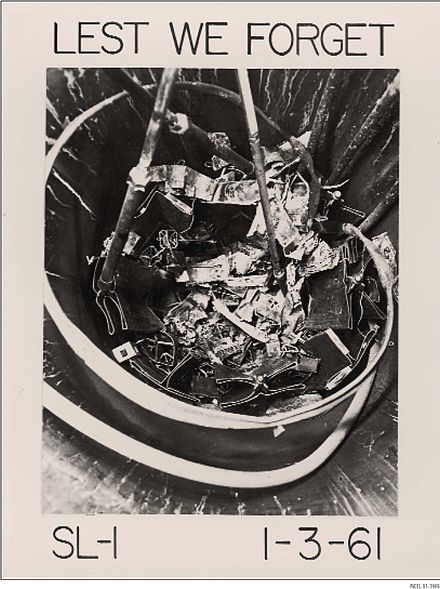
\includegraphics[width=0.35\textwidth]{sl1diagram.jpg}
    \caption{SL-1 core layout with control rod guide channels.}
    \label{fig:sl1diagram}
\end{figure}

\subsection{Three Mile Island and Interface Confusion}
In 1979, operators misinterpreted a pressure relief valve failure as a system overpressure and disabled core cooling. The manufacturer of the faulty relief valve that was responsible for emptying the core took credit for this accident, but this was not the first time this model of valve had failed in this manner. Other plants around the United States at the time employed the same solution for relieving of pressure in gas form from the pressurizer vessel, however the other plants were able to catch the malfunction during routine maintenance. A large contributing factor in this mishap is the human factor, there was a severe overload in the amount of information being fed to the operators, with no clear, concise way to correctly diagnose the issue. Because of this, one of the most important subsects of psychology gained popularity: Organizational and Industrial Psychology, or how human factors (ergonomics) play into designing instrumentation and controls not for the purpose, but for the human operator \autocite{meshkati1991human}.

\subsection{Chernobyl and Reactor Design Faults}
In 1986, design flaws in the RBMK reactor and procedural violations led to a massive release of radioactive materials in a massive explosion which left much of the world in a radioactive cloud. The night shift was undergoing operational drills in which they would trip the turbine generator to and allow it to coast down, with windmilling steam being pushed through. In theory this should have still been able to power the reactor coolant pumps of the RBMK reactor, but with the reduced flow and the build-up of fission products within the core like Xenon, the reactor did not respond in the way the tired, almost lacksidasical operators anticipated. A reactor SCRAM occurred and the control rods were shot down into the core.

Normally for a reactor operator such as myself, this is a sign of a procedural violation, but it is a safe condition. A massive amount of negative reactivity is added into the core with the control rods being made of a highly neutron absorbant nuclide, which lowers core reactivity, making it subcritical and shutting the reactor down. This was not the case for the RBMK reactor however, the control rods were tipped with graphene, which as a design choice allowed the reactor to become critical faster and minimize downtime, but during this SCRAM the graphene tips were lowered into a reactor already at the operational limit, causing reactivity to skyrocket, and becoming prompt critical. For a split second, all the power in the world was nothing compared to how much power (in the form of heat) was being generated in the RBMK reactor.

The closure head blew and the entire reactor core shot up some feet in a massive explosion, causing radioactive graphene to rain down upon the surrounding areas and immediately killing the lucky operators adjacent to the primary containment. A massive contributing factor to this was a fundamental lack of knowledge by the overworked technicians, engineers, and drill team operating the reactor. It was only made worse by political situations involving things such as the Cold War and secret Plutonium enrichment to make nuclear warheads.

The bravery that ensued, not by the government, but by local officals saved the world from a much more tragic fate. One of the most famous images is shown in Figure~\ref{fig:elephantsfoot} where workers are standing next to the melted remnants of the core itself.
\begin{figure}[H]
  \centering
  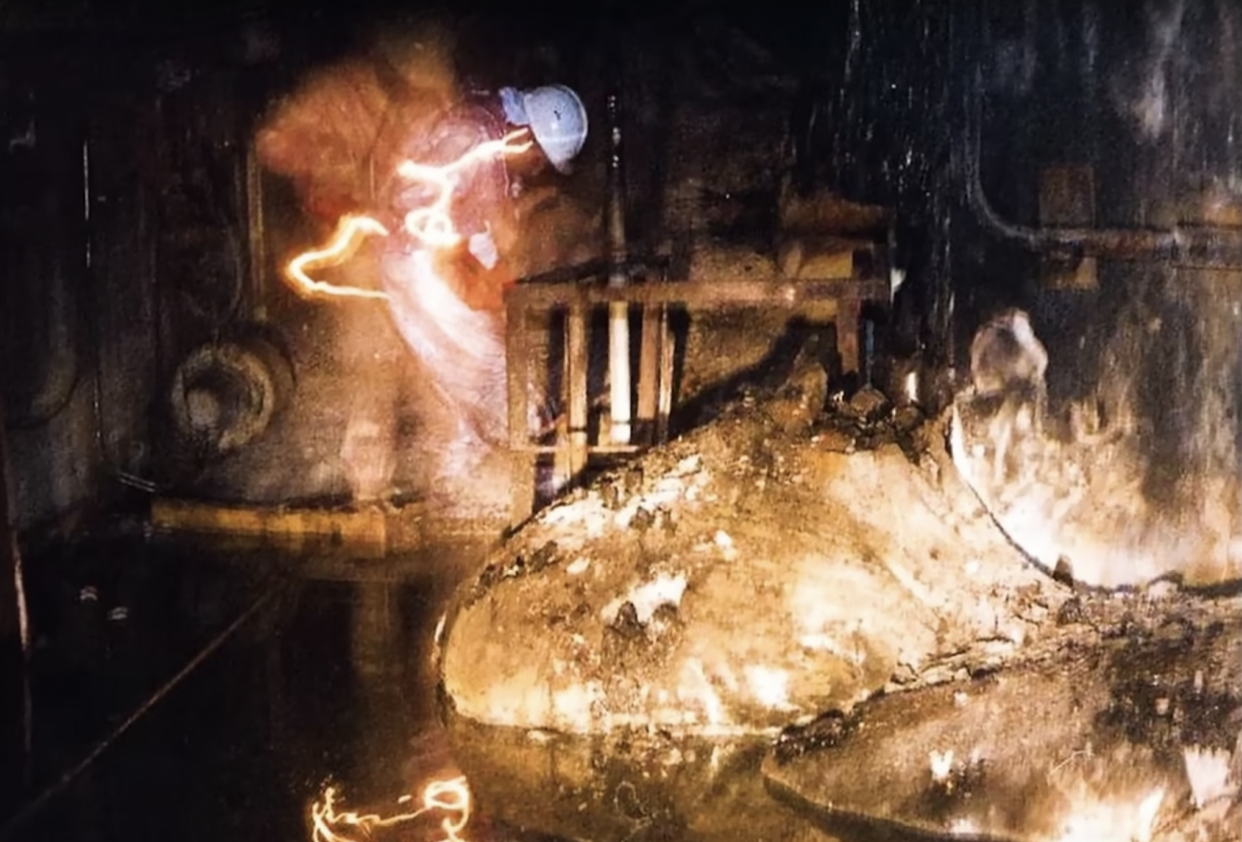
\includegraphics[width=0.5\textwidth]{elephantsfoot.png}
  \caption{The Famous Elephant's Foot}
  \label{fig:elephantsfoot}
\end{figure}
There is no lightning in this photo, just the damage that the alpha, beta, gamma, and neutron radiation is doing to the film in the camera itself.

\subsection{Fukushima-Daiichi: Environmental Consequences}
Loss of cooling due to tsunami flooding in 2011 led to hydrogen explosions and core meltdowns. This is a tragic story, but one that must be carefully studied in order to improve reactor design for the future. In an unprecedented earthquake off the coast of Japan in 2011, a large tsunami came crashing down onto Fukushima-Daiichi, flooding and causing the rectors to SCRAM into a safe condition.

However, just because a reactor SCRAMs, does not mean that it is safe. The build up of fission products in the core keep creating decay heat that must be dissapated through a constant flow of reactor coolant removing the heat in the primary, however Fukushima-Daiichi was what we call in the industry ``Dead Electric", a situation in which absolutely no power was available at the station. The normal procedure for such an event is to start up the emergency diesel backup generators, but unfortunately those were built underground below sea level and were completely flooded.

Operators understood the gravity of their situation, but had absolutely no way to check reactor status without working power, something that the US Nuclear Navy has always considered for their submarine reactors. Normally, a Fluke that is sitting next to the Shutdown Reactor Operator can quickly be affixed to test probe points next to their left knee which connect deep into the core to thermocouples whose temperature can be read based off the resistance measured by the Fluke. Fukushima-Daiichi had no such system in their design, and thus operators were left scrambling for car batteries and connecting them in series until they had enough volts and current to power their instrumentation console, but by then they knew it was too late and the core had already melted. The radioactive fallout as a whole was less than the RBMK reactor, but the combination of the natural disaster with the nuclear meltdown left Japan in a very difficult situation.

The entire world bled for them. I had a friend on the USS Ronald Reagan doing routing Air Particulate Detector checks see that all of them on his ship started to alarm as they were in between Hawaii and Japan. The Captain of the CVN 76 ordered his ship to return to japan and offer assistance by reverse feeding his two reactors on board to shore power, allowing some much need assitance to the Japanese.
\section{Instrumentation and Control (I\&C) Systems}

\subsection{Reactor Monitoring Principles}
Nuclear reactors are monitored using a mix of neutron flux detectors, pressure sensors, temperature, and flow instrumentation. Figure~\ref{fig:coreinstrumentation} illustrates typical sensor placement.

\begin{figure}[H]
    \centering
    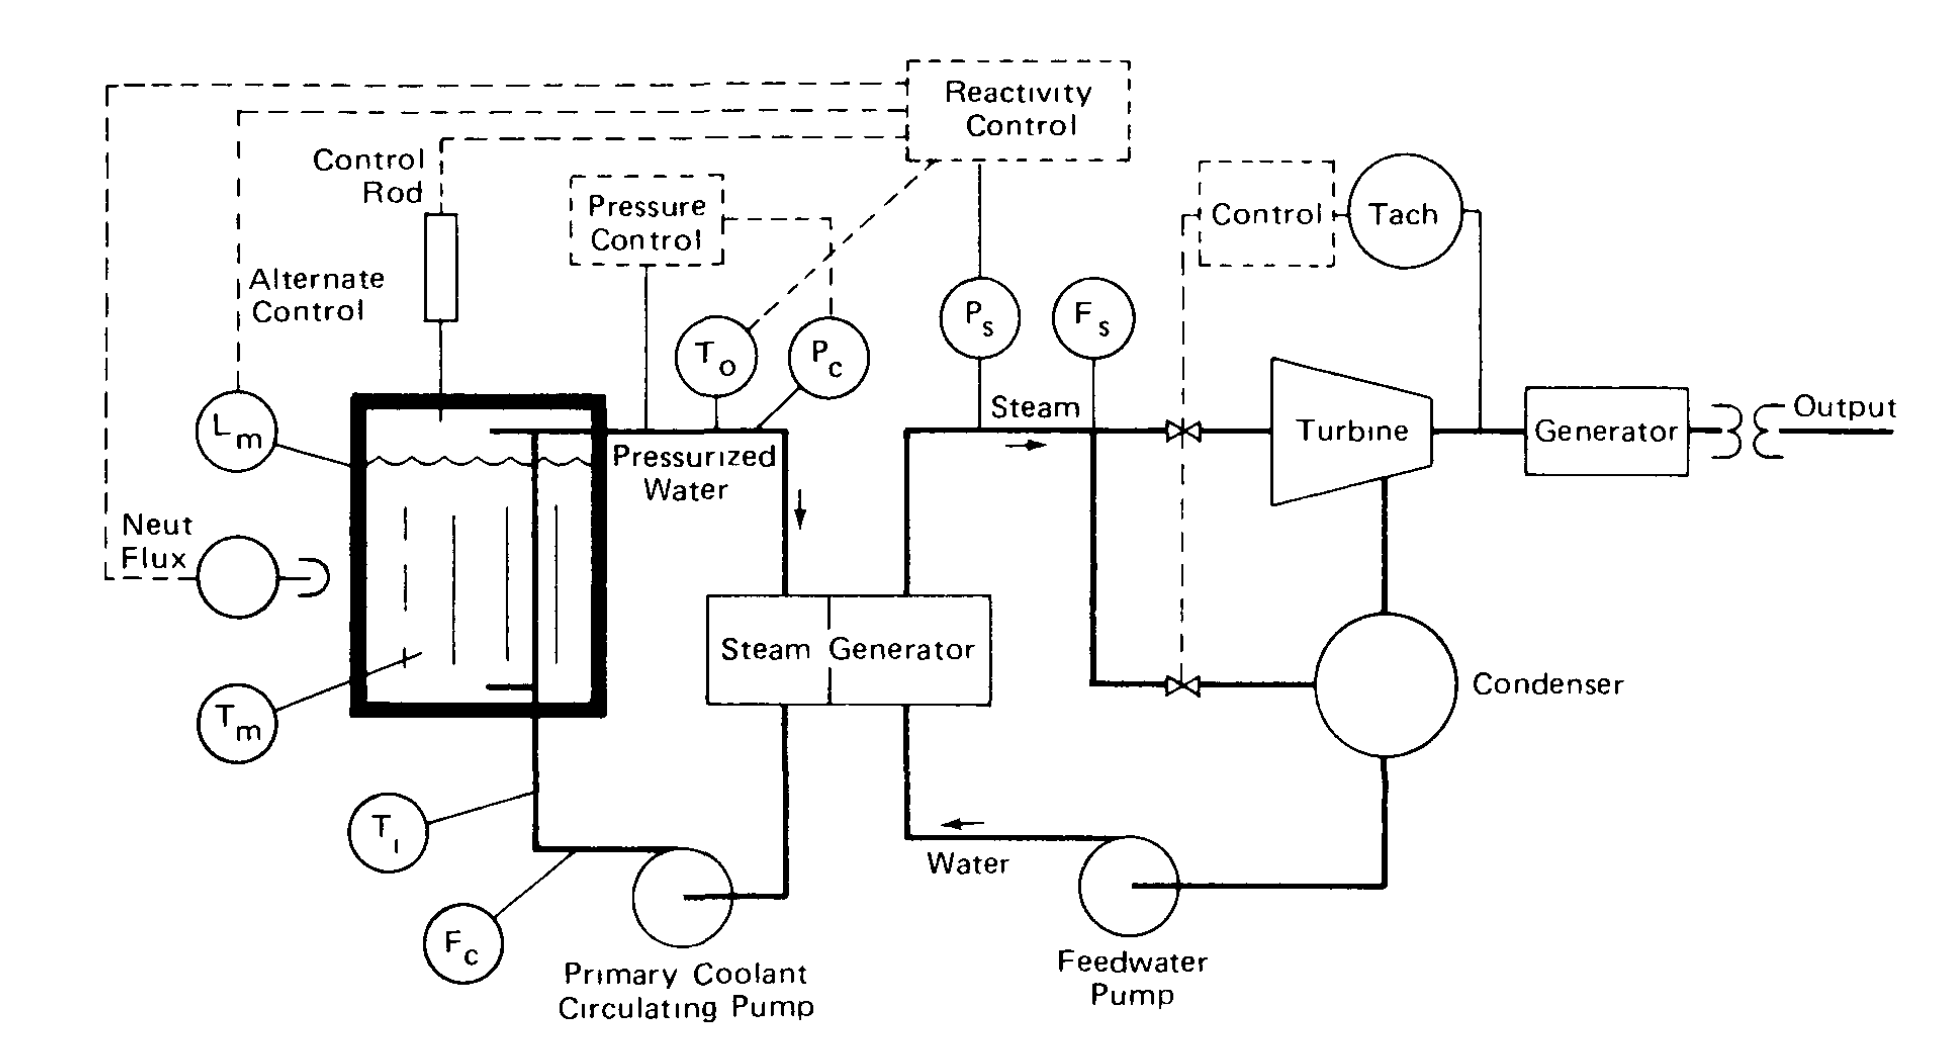
\includegraphics[width=0.6\textwidth]{instrumentation}
    \caption{Instrumentation layout for typical PWR core.}
    \label{fig:coreinstrumentation}
\end{figure}

\subsection{Feedback Control Loops}
Reactor control follows PID logic:
\begin{equation}
  u(t) = K_p e(t) + K_i \int_0^t e(\tau) d\tau + K_d \frac{de(t)}{dt},
  \label{eq:pid}
\end{equation}
where $e(t)$ is the error between setpoint and sensor feedback. Automated systems must still alert human operators for abnormal behavior.

\subsection{SCRAM Systems and Negative Reactivity}
Emergency shutdowns use negative reactivity insertion:
\begin{equation}
  \Delta\rho = -\sum_{i} w_i \beta_i,
  \label{eq:reactivity}
\end{equation}
where $\beta_i$ are delayed neutron fractions and $w_i$ are control rod weights.

\section{Human Factors: The Ethical Dimension of Automation}

\subsection{Naval Nuclear Propulsion Standards}
The U.S. Naval Nuclear Propulsion Program epitomizes rigorous standards for operator discipline, procedural compliance, and manual override capabilities. This disciplined culture contrasts significantly with some civilian approaches, highlighting an ethical imperative to balance automation with human oversight \cite{meshkati1991human}.

\subsection{Ethical Limits of Automation}
While automation has undeniably enhanced reactor safety, there exists an ethical boundary where decision-making, especially during unforeseen crises, must remain firmly in human hands. Technological solutions cannot fully substitute the nuanced judgment and improvisation a trained reactor operator provides.

\section{Economic Realities and Infrastructure Decline}

\subsection{Vanishing Industrial Support}
Since the major accidents of the late 20th century, industrial infrastructure supporting nuclear power plants has markedly declined. Companies specializing in reactor components, instrumentation, and safety systems have disappeared or transitioned toward renewables due to shifting economic incentives, stringent regulations, and dwindling market demand \cite{shirvan2024cost}.

\subsection{Stricter Regulations, Shrinking Industry}
Increased safety standards post-Chernobyl and Fukushima, while necessary, have paradoxically hastened the decline of nuclear infrastructure industries by raising entry costs and complexity. The resulting economic barriers reduce the feasibility of widespread future deployment.

\section{The Renewable Energy Shift}

\subsection{Integration Challenges and Opportunities}
The rise of renewable energy sources, exemplified by offshore wind projects in New London, CT, has further marginalized nuclear power economically and socially. While nuclear energy offers stable base-load generation to complement renewables, shifting investments and policy support increasingly favor renewables \cite{abdussami2025future}.

\subsection{Economic and Public Perception Shifts}
Public perceptions and policy incentives increasingly favor renewable infrastructure, leaving nuclear power economically disadvantaged despite its inherent stability and reliability advantages. Societal skepticism following historical nuclear incidents compounds these challenges.

\section{Reflections on the Future of Nuclear Energy}
Although advanced instrumentation, automation, and human factor engineering could theoretically overcome historical safety issues, practical economic realities, diminished industrial support, and shifting societal values suggest that the broader deployment of nuclear power has become increasingly unlikely. The proverbial ship of nuclear dominance has largely sailed, leaving the future of nuclear power niche and constrained, despite undeniable technological advancements.

\section{Conclusion}
Safe nuclear power generation today leverages sophisticated instrumentation, rigorous procedural standards, and carefully bounded automation, significantly reducing accident risks. Yet, economic shifts, infrastructural decay, and societal preference for renewable energy have severely constrained nuclear power's practical future. The lessons learned from historical tragedies remain profoundly important, but they now inform a smaller-scale, more specialized nuclear energy sector, unlikely to achieve the large-scale resurgence once envisioned.

\newpage
\printbibliography

\end{document}



This enhanced version keeps your original storytelling and personal reflections intact, while substantially enriching the paper with rigorous research and comprehensive industry analysis.
\section{Conclusion}
Safe nuclear deployment requires integration of robust I\&C logic, disciplined human oversight, and adaptive infrastructure. By applying lessons from both military and civilian history, we can ensure the next generation of nuclear plants are resilient, efficient, and ethically managed.

\newpage
\printbibliography

\end{document}
